\documentclass[10pt,french]{book}
\input preambule_2013

\newcounter{exoc}
\newenvironment{exoc}[1]{%
  \refstepcounter{exoc}\textbf{Exercice \theexoc} :\hfill {\textbf{(#1)}}\par
  \medskip}%
{\medskip}

\pagestyle{empty}

\begin{document}

\begin{center}
\begin{tabularx}{\textwidth}{|>\centering m{2.5cm}|>\centering X|>{\centering\arraybackslash} m{2.5cm}|}
	\hline
		\seconde 7 &  Jeudi 14 novembre \np{2013} & \textbf{Coordonnées Fonctions} \\
	\hline
		\multicolumn{3}{|c|}{\bsc{Contrôle de mathématiques}} \\
	\hline
        \multicolumn{1}{|r}{\bsc{Nom}:} & \multicolumn{2}{l|}{} \\
		\multicolumn{1}{|r}{Prénom:} & \multicolumn{2}{l|}{} \\
	\hline
        \multicolumn{3}{|l|}{\bfseries Note et observations :} \\[1cm]
    \hline
\end{tabularx}\bigskip

{\itshape
La qualité et la précision de la rédaction seront prises en compte dans l'appréciation des copies.
Le barème est indicatif.}
\end{center}

\begin{exoc}{3 + 1 + 3 + 1 = 8 pts}
    Dans un repère orthonormé \OIJ, on considère les points suivants :
    \[A(2\pv 1) \qq B(3 \pv 2) \qetq C(1 \pv 3).\]
    \begin{enumerate}
        \item Démontrer que le triangle $ACB$ est isocèle en $C$.
        \item Calculer les coordonnées du milieu $M$ du segment $[BC]$.
        \item On considère maintenant le point $D$ tel que $ABDC$ et un parallélogramme.
            \begin{enumerate}
                \item Quel est le milieu du segment $[AD]$ ? Justifier précisément.
                \item Calculer alors les coordonnées du point $D$.
            \end{enumerate}
        \item Sans calcul, déterminer la longueur $[BD]$. Justifier précisément.
    \end{enumerate}
\end{exoc}

\begin{exoc}{0,5+1+1,5+1 = 4 pts}
    On a enregistré la vitesse en \SI{}{km/h} d'une voiture roulant en ville durant une minute. On définit donc la fonction $T$ qui, à un temps $t$ donné, associe la vitesse $v$ :
    \begin{center}
        \begin{tabular}{|>\bfseries c|*{7}{>{\centering\arraybackslash}m{0.5cm}|}}
            \hline
                Temps (en \SI{}{s}) & $0$ & $10$ & $20$ & $30$ & $40$ & $50$ & $60$ \\
            \hline
                Vitesse $v$ (en \SI{}{km/h}) & $15$ & $25$ & $40$ & $0$ & $10$ & $25$ & $50$ \\
            \hline
        \end{tabular}
    \end{center}
    \begin{enumerate}
        \item La fonction $T$ est-elle définie pour $t = 15$ ? Pourquoi ?
        \item Donner les antécédents de $25$. Interpréter les résultats en s'aidant du contexte du problème.
        \item Donner l'image de $10$ par la fonction $T$. Interpréter le résultat en s'aidant du contexte du problème.
        \item Donner un nombre qui n'a pas d'image et un nombre qui n'a pas d'antécédent. Expliquer le raisonnement.
    \end{enumerate}
\end{exoc}

\begin{exoc}{1pt par question : 8 pts}
Dans un repère \OIJ, on a tracé la courbe $\calig C_f$ représentative de la fonction $f$.

\begin{minipage}{0.6\textwidth}
    \begin{description}
        \item[Partie A :] Par lecture graphique.
           \begin{enumerate}
                \item Déterminer $f(0)$ et $f(-2)$.
                \item Quels sont les antécédents du nombre $1$ ?
                \item Quels sont tous les nombres qui ont $3$ antécédents par $f$ ? Donner la réponse sous forme d'un intervalle.
            \end{enumerate}
        \item[Partie B :] Par calcul numérique.\par La fonction $f$ est définie pour tout $x \in \R$ par \[f(x) =\frac 12 \left(4x^3 - 3x + 1\right).\]
            \begin{enumerate}
                \item Le point $E$ de coordonnées $(-1,25 \pv -1,5)$ appartient-il à $\calig C_f$ ? Justifier la réponse.
                \item Calculer $(2x - 1)^2$.
                \item Démontrer que $4x^3 - 3x + 1 = (x + 1)(2x - 1)^2$.
                \item En déduire les antécédents de $0$ par la fonction $f$
                \item Calculer l'image de $\frac 1 2$ par la fonction $f$. Donner le résultat sous forme fractionnaire.
            \end{enumerate}
    \end{description}
\end{minipage}\hfill
\begin{minipage}{0.35\textwidth}
    \begin{center}
        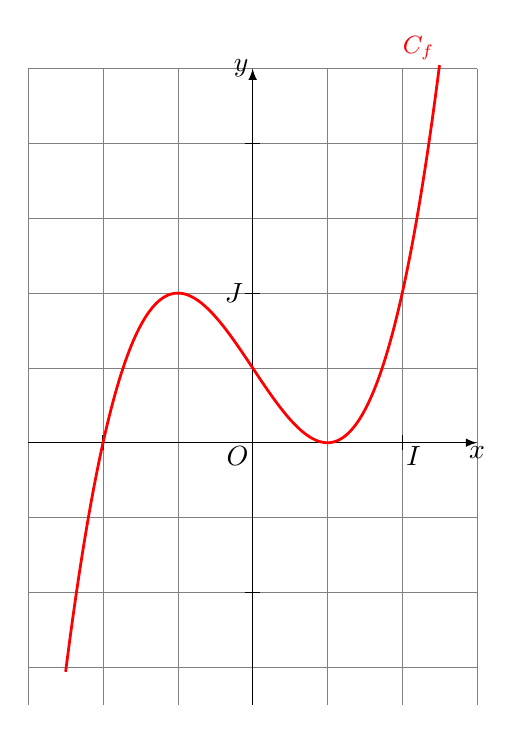
\begin{tikzpicture}[>=latex,y=2cm,x=2cm,scale=0.95]
            \draw[help lines] (-1.5,-1.75) grid (1.5,2.5);
            \draw[->] (-1.5,0) -- (1.5,0) node[below=-2pt] {$x$};
            \draw[->] (0,-1.75) -- (0,2.5) node[left=-2pt] {$y$};
            \coordinate (O) at (0,0); \draw (O) node[below left = -2pt] {$O$};
            \coordinate (I) at (1,0); \draw (I) node[below right = -2pt] {$I$}; \foreach \x in {-1,...,1}  \draw (\x,-0.05)--(\x,0.05);
            \coordinate (J) at (0,1); \draw (J) node[left] {$J$}; \foreach \x in {-1,...,2} \draw (-0.05,\x)--(0.05,\x);
            \draw[color=red,line width=1pt] plot[domain=-1.25:1.25,samples=200] (\x,{(4*(\x)^3-3*\x+1)/2}) node[above left=-2pt] {\small $\calig C_f$};
        \end{tikzpicture}
    \end{center}
\end{minipage}
\end{exoc}
\end{document} 



\begin{center}
    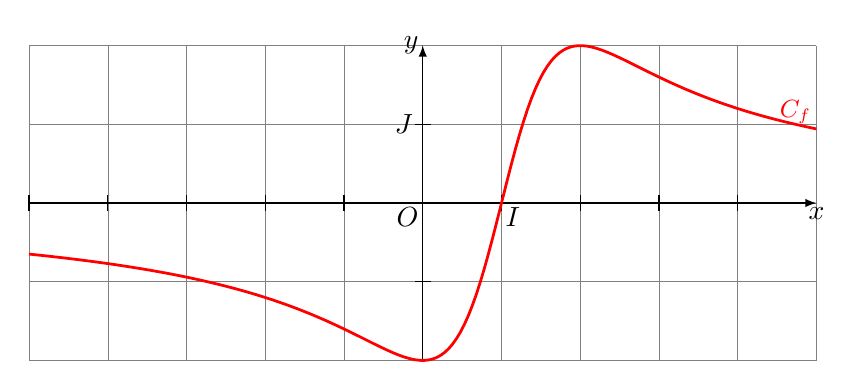
\begin{tikzpicture}[>=latex]
        \draw[help lines] (-5,-2) grid (5,2);
        \draw[->] (-5,0) -- (5,0) node[below=-2pt] {$x$};
        \draw[->] (0,-2) -- (0,2) node[left=-2pt] {$y$};
        \coordinate (O) at (0,0); \draw (O) node[below left = -2pt] {$O$};
        \coordinate (I) at (1,0); \draw (I) node[below right = -2pt] {$I$}; \foreach \x in {-5,...,4}  \draw (\x,-0.1)--(\x,0.1);
        \coordinate (J) at (0,1); \draw (J) node[left] {$J$}; \foreach \x in {-2,...,1} \draw (-0.1,\x)--(0.1,\x);
        \draw[color=red,line width=1pt] plot[domain=-5:5,samples=200] (\x,{4*(\x-1)/((\x-1)^2+1.001)}) node[above left=-2pt] {\small $\calig C_f$};
    \end{tikzpicture}
\end{center}